\chapter{Background}
\section{Cyber Physical Systems}
\subsection{Hybrid Systems}
A system with both continuous (frequently physical) components and discrete (frequently digital)
components is said to be a \emph{hybrid system}, named for its characteristic blending of the
two domains. Examples of hybrid computer systems abound in industrial controls, for example,
although hybrid systems may also be fully physical (e.g., a bouncing ball experiences continuous
behavior when rising and falling and discrete behavior when colliding with a surface).

The term hybrid system is an older one that was coined as researchers began to study the newly
pervasive reactive systems that arose as programmed control of the physical world became 
widespread ~\cite{alur1993hybrid}. For several reasons it does not suffice to describe precisely
the types of systems with which this work is concerned: a subset of hybrid
systems that incorporate a significant computer and networking component.

Nevertheless, the modeling of hybrid systems is well studied and provides a sufficient body
of relevent knowledge from which to draw to warrant its inclusion. This chapter includes
background on a particularly relevent modeling framework for hybrid systems called the
hybrid automaton, which is used in this thesis as the standard benchmark against which to
compare hybrid modeling techniques.
\subsection{Cyber Physical Systems}
\subsubsection{Definition}
% Definition
A newer, better term for the systems investigated in this thesis is \emph{cyber physical systems}.
Put simply, a cyber physical system is a networked hybrid system: a networked computer system that is 
tightly coupled to the physical world. 
\subsubsection{Challenges}
According to the 2008 Report of the Cyber-Physical Systems Summit, ``The principal barrier to 
developing CPS is the lack of a theory that comprehends cyber and physical resources in a 
single unified framework.''~\cite{summitreport2008}

The summit further identified as part of the scientific and technological foundations of
cyber physical systems both new modeling frameworks that ``explicitly address new observables'' and 
studies of privacy, trust, and security including ``theories of cyber-physical inter-dependence''~\cite{summitreport2008},
a major theme of this work.

Crenshaw and Beyer enumerated four principal challenges in cyber physical systems testing that are
equally apt for security:
their concentration in safety critical domains, their frequent integration of third-party or
otherwise unrelated systems, their dependence upon unreliable data collection, and their
pervasiveness~\cite{crenshaw2010upbot}.
\subsection{Hybrid Automata}
\subsubsection{Definition}
A valuable formalism for modeling hybrid systems in isolation and with limited composition
is the hybrid automaton of Alur, et al.~\cite{alur1993hybrid}. This section introduces the
version of the formalism described in 1996 by Henzinger~\cite{henzinger1996theory}, to which a
reader interested in more than a superficial understanding is referred. 

Formally,
a hybrid automaton $H$ is made up of a set of real-valued state variables, their first derivatives,
a set of operational modes and switches between the modes, and predicates attached to those modes and
switches describing the operation of the system in those modes and the discrete transitions between
them. One can think of a hybrid automaton as a pairing of a finite state machine whose states (called
modes) and transitions (called switches) denote the discrete-domain behavior of the hybrid system, with
a set of differential equations attached to each mode, which govern its continuous-domain behavior. Switches
may also be labeled in order to permit synchronization across composed hybrid automata.

Modes may be decorated with invariant conditions (which state whether the system is allowed to be in that mode),
flow conditions (which state how the continuous domain state variables are permitted to evolve while in that
mode), and initial conditions (which state under which, if any, conditions the automaton may begin its operation
with that mode). Switches are decorated with jump conditions, which serve as guards on the switch determining
both (1) when the switch is allowed to be taken, and (2) the discrete changes in state variables due to that
switch's activation.

A simple example of a hybrid automaton is given in Fig.~\ref{fig:thermostat}, which models a simple
heater thermostat. The nodes in the automaton represent its operating modes, and the edges represent
switches. In the ``Off'' mode, the temperature (given by $x$) must be greater than or equal to 18, and
its first derivative with respect to time (denoted $\dot{x}$) is $-0.1x$, which represents a cooling of
the environment. When the temperature is strictly less than 19, the switch from off to on is available (but
not mandatory until the off mode's invariant condition $x \geq 18$ ceases to be satisfied. The switch from
on to off behaves similarly.

\begin{figure}
\centering
\begin{dot2tex}[options=-t raw --autosize]
digraph G {
    rankdir=LR;
    
    Off [texlbl="$\begin{matrix} \text{Off} \\ \
    \dot{x} = -0.1x \\ \
    x \geq 18 \\ \
    \end{matrix}$"];
    
    On [texlbl="$\begin{matrix} \text{On} \\ \
    \dot{x} = 5 - 0.1x \\ \
    x \leq 22 \\ \
    \end{matrix}$"];
        
    Off -> On [label=" " texlbl="$x < 19$"];
    
    On -> Off [label=" " texlbl="$x>21$"];
}
\end{dot2tex}
\caption{Thermostat hybrid automaton~\cite{henzinger1996theory}}
\label{fig:thermostat}
\end{figure}

The hybrid automaton model is sufficiently rich to capture many hybrid systems. 
\subsubsection{Shortcomings}
There are some problems with the hybrid automaton model. A hybrid automaton is not guaranteed to
have a valid execution, and computing whether it does or not is non-trivial~\cite{lygeros1999existence}.
Model checking has been developed for only some subclasses of 
automata~\cite{henzinger1997hytech}~\cite{frehse2005phaver}, and many desirable
properties of them are undecidable~\cite{henzinger1998s}.

However, there are even more nagging problems when considering hybrid automata or their variants
for the study of cyber physical systems. One of the hallmarks of cyber physical systems is a
distributed and highly networked nature. While they provide a
natural model for the discrete-continuous boundary, hybrid automata have only a rudimentary
notion of communication, no clear means for specifying message passing, and when used in large
topologies have significant scaling problems, both computationally and cognitively.
\subsubsection{Alternatives}
Some attempts have been made to solve the problem of the hybrid automaton's unsatisfactory
capability for modeling networks and communication. Particularly, the designation of shared
actions and shared variables as ``input'' or ``output'' is a popular tactic, used in the
powerful hybrid I/O automaton~\cite{lynch1996hybrid}~\cite{lynch2001hybrid}, its descendent the
timed I/O automaton~\cite{kaynar2010theory}, and also in the PHAVer model 
checker~\cite{frehse2005phaver}.

The work of this thesis is also something of an outgrowth from an instance of this strategy in
which prototypical ``hybrid link automata'' were developed to model explicit communication channels.
An example of the cognitive scalability issues inherent with this design is given in Fig.~\ref{fig:linkmachine}.
This strategy may have a place in modeling some systems but falls short of the goal of 
modeling complex, interdependent networks of hybrid systems with more conventional computer networks.
\begin{figure}
\centering
\begin{dot2tex}[options=-t raw --autosize]
digraph G {
    rankdir=LR;
    idle [shape=circle, texlbl= \
    "$ \begin{matrix} \lambda : \mu : \text{Idle} \\ \
    \dot{C}_{\lambda \mu} = 0 \\ \
    C_{\lambda \mu} = 0 \end{matrix} $"];
    
    transmit [shape=circle, texlbl= \
    "$ \begin{matrix} \lambda : \mu : \text{Transmit} \\ \
    \dot{C}_{\lambda \mu} = 1 \\ \
    C_{\lambda \mu} < l \wedge w_{\lambda}=1  \end{matrix}$"];
    
    wait [shape=circle, texlbl= \
    "$\begin{matrix} \lambda : \mu : \text{Wait} \\ \
    w_{\lambda}=1 \\ \
    \end{matrix}$"];
    
    transmit -> idle [label= " " \
    texlbl="$\begin{matrix} \lambda : D : \mu \\ \
    C_{\lambda \mu} < l \\ \
    C_{\lambda \mu} := 0 \wedge w_{\lambda}:=0 \
    \end{matrix}$"];
    
    idle -> transmit [label= " ", \
    texlbl= "$\begin{matrix} S : \lambda : \mu \\ \
    w_{\lambda}=0 \\ \
    w_{\lambda}:=1 \\ \
    \end{matrix}$"];
    
    idle -> wait [label= " ", \
    texlbl= "$\begin{matrix} S : \lambda : \mu \\ \
    w_{\lambda}=1 \\ \
    \end{matrix}$"];
    
    wait -> transmit [label= " ", \
    texlbl= "$\begin{matrix} \
    w_{\lambda}=0 \\ \
    w_{\lambda}:=1 \\ \
    \end{matrix}$"];
    
    wait -> wait [label= " ", \
    texlbl= "$\begin{matrix} S : \lambda : \mu \\ \
    \end{matrix}$"];
    
    idle -> idle [label= " ", \
    texlbl="$\lambda : D : \mu$"];
    
    idle -> transmit;
    
    transmit -> idle;
    idle -> idle [label= " ", \
    texlbl="$S : \lambda : \mu$"];
    
}
\end{dot2tex}
\caption{An example of a considered ``hybrid link automaton'' prototype modeling
a link on which messages may be dropped, injected, or delayed, and on which mutual
exclusion of messages is enforced.}
\label{fig:linkmachine}
\end{figure}
\section{Attack Graphs}
\subsection{Introduction}
An attack graph is one of several related formalisms that utilize graph theory to
model the state space of computer systems attacks. Perhaps they are best introduced
when presented as an alternative to a similar model called an attack tree.
\subsection{Attack Trees}
An attack tree is a goal-oriented tree model of an abuse of a system~\cite{schneier1999modeling}.
The root of the tree represents the attacker's goal, and the children of any given node represent
the prerequisite activities required to reach that node. For example, consider the goal of
stealing a car, which is modeled in a simple attack tree in Fig.~\ref{fig:attacktree}.

The attacker must start the car and drive away; this could be accomplished either by breaking
in and hotwiring the car, or by stealing the owner's key and using it to subsequently steal the
car. The root of the tree represents the final goal of the theft, with prerequisite goals
flowing upward from the leaf nodes.
\begin{figure}
\centering
\begin{dot2tex}[options=-t raw --autosize]
digraph G {
    rankdir=BU;
    StealCar [label="Steal car"];
    UseKey [label="Start car with key"];
	HotWire [label="Hotwire car"];
	StealKey [label="Steal owner's key"];
	OpenDoor [label="Access car interior"];
	CallLocksmith [label="Impersonate owner to locksmith"];
	BreakWindow [label="Break in through window"];
	UseKey -> StealCar;
	HotWire -> StealCar;
	StealKey -> UseKey;
	OpenDoor -> HotWire;
	CallLocksmith -> OpenDoor;
	BreakWindow -> OpenDoor;
}
\end{dot2tex}
\caption{Simple car theft attack tree}
\label{fig:attacktree}
\end{figure}

There are a few features of this modeling method to note. It is goal oriented, meaning that
the consequences of the attack are known, and the goal is to ennumerate and and analyze the
means by which those consequences could be reached. It is, as an attack model, agnostic to the
underlying system model which makes it difficult to generate automatically. Finally, and perhaps
most significantly, it captures the ways in which an attacker's actions interact and 
depend upon each other.

This threat-centric model is not necessarily the most useful for system stakeholders. It
requires, in a sense, that one work backward from the attack to the system state
necessary to realize the attack. If, instead, an analyst desires to work from a system characterization
and explore the attack space permitted by that system characterization, the attack tree framework
must be in some sense turned upside down. 
Attack graphs do exactly that.
\subsection{Attack Graphs}
\subsubsection{Introduction}
In contrast to attack trees, attack graphs permit a topology-aware exploratory analysis of
the state space of a system. It is a graph theoretic model in which vertices represent individual
system states, and edges represent state transitions caused by an adversary. The concept as
introduced in 1998 included notions of generalized attack patterns to be bound to state transitions;
network elements and their individual configurations; network topology (three characteristics common
to all current attack graph iterations); a notion of the attacker's capabilities, and edge weights
representing likelihood~\cite{phillips1998graph}. A similar structure called a privilege graph was
introduced in 1994~\cite{dacier1994privilege}.

Most approaches to attack graph modeling represent exploits (attack patterns) as using
preconditions and postconditions~\cite{lippmann2005annotated} since this was suggested in about 2000~\cite{templeton2001requires}. Exploits are chained together by matching preconditions in a state node's
underlying system model and applying their postconditions to generate a successor state.
\subsubsection{Model Types}
The modeling substrates of attack graphs can be broadly separated into two schools of
thought, separated by the philosophy that guides the representation of the underlying
network model over which network states and transitions are computer.

A specification of an underlying network model may be done with only very loose
restrictions, allowing arbitrary keywords as named qualities and topoligies of network objects.
This thesis employs this method. It is also favored in the work of George Mason 
University~\cite{ammann2002scalable}~\cite{wang2006minimum}. It has the advantage of
permitting more straightforward adaptation into the continuous domain, which is the reason
it is favored by this work. 

An alternate specification method is much more restricted, confining the modeler to
certain sets of terms imposing explicit computer networking comcepts onto the model~\cite{templeton2001requires}.
This permits generation and analysis to take advantage of networking concepts to perform a
more nuanced analysis of a network state, including reachability analysis to determine whether a
given topology permits communication between two hosts~\cite{ingols2009modeling}. This approach
is favored, for example, in the work of MIT Lincoln Laboratory and the University of California, Davis.
\subsubsection{Generation}
Methods of attack graph generation, the process of chaining exploits to enumerate the
attack space~\cite{campbell2002modeling}~\cite{phillips1998graph}~\cite{sheyner2002automated},
share a common general architecture among the modern
methods that use preconditions and postconditions in exploit definitions,
pictured in Fig. \ref{fig:generation}. The attack graph generation
process combines network state and exploit patterns as input, applying exploit postconditions
back onto the network state to generate its output of successor states.

\begin{figure}
\centering
\begin{dot2tex}[options=-t raw --autosize]
digraph G {
	rankdir=TD;
    Generator [texlbl="Generation Engine", shape="rectangle"];
    Exploits [texlbl="\begin{tabular}{c}Exploit Rules\\ (Generic transitions)\end{tabular}", shape="ellipse"];
	State [texlbl="\begin{tabular}{c}Network State\\ (Facts)\end{tabular}", shape="ellipse"];
	Exploits -> Generator [texlbl="\begin{tabular}{c}1a. Read exploit \\ preconditions\end{tabular}" label=" "];
	State -> Generator [texlbl="\begin{tabular}{c}1b. Match preconditions \\ with network state\end{tabular}" label=" "];;
	Generator -> State [texlbl="\begin{tabular}{c}2. Apply new\\ network state\end{tabular}" label=" "];
}
\end{dot2tex}
\caption{Attack graph generation process}
\label{fig:generation}
\end{figure}
\subsubsection{Research Directions}
Research in attack graphs is spread throughout a variety of pathways. Many of these include
evaluating a network's security~\cite{ammann2002scalable}, specification of formal languages
to represent attack graphs~\cite{templeton2001requires}, intrusion detection system 
integration~\cite{tidwell2001modeling}, automatic generation of security recommendations~\cite{wang2006minimum},
and reachability analysis between hosts in a single network state~\cite{ingols2009modeling}. 
For a thorough literature review up to 2005 and more detailed discussion of popular research directions, 
refer to the work of Lippmann and Ingols~\cite{lippmann2005annotated}.
\section{Case Studies}
Throughout this thesis, two examples of attacks are used to illustrate the models presented.
The first is on a traditional information system, based upon an offensive educational exercise
deployed at the University of Tulsa in 2008 involving several chained attacks. The second is the 
denial of service through battery exhaustion of a simple
cyber-physical system of active radio frequency identification (RFID) tags and readers.
\subsection{Blunderdome}
The first case study is an attack on a simulated educational network deployed as part of a
security engineering course in 2008. Dubbed the Blunderdome, it featured a firewalled network of
two hosts available per attacker. See Table \ref{table:blundertasks} for a listing of the stages and
their preconditions and results. The attacker was required to log into a login server by cracking
its weak SSH key (due to an operating system vulnerability), execute an elevation of privilege (due
to a Linux kernel vulnerability), log into the web server, and execute a SQL injection attack to
change a simulated grade. The architecture from the exercise is provided in 
Fig.~\ref{fig:blunderarch}~\cite{louthan2010blunderdome}.

\begin{figure}
\centering
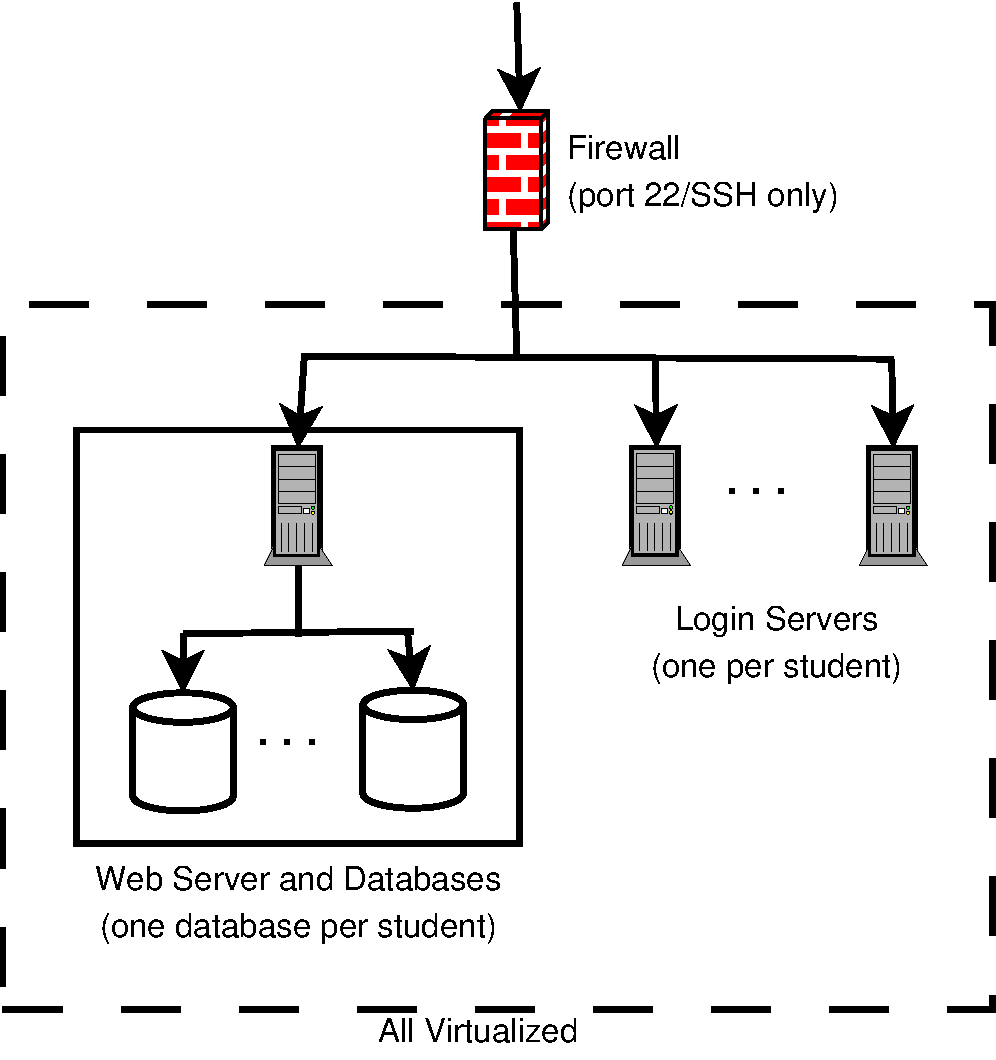
\includegraphics[width=3in]{blunderarch}
\caption{Blunderdome network architecture}
\label{fig:blunderarch}
\end{figure}

\begin{table}
\centering
\begin{tabular}{p{1.5in}|p{1in}|p{1in}|p{1in}}
Stage & Precondition	&	Attack	&	Postcondition \\ \hline \hline
Gain remote user access & SSH public key available (given); weak public key 
	& Break weak public key & User privileges on login server \\ \hline
Gain root access & User-level access & Execute \texttt{vmsplice} privilege escalation 
	& Root privileges on login server; access to web server credentials \\ \hline
Change grade & Address and credentials for web service & Execute SQL injection & Altered grade in database
\end{tabular}
\caption{Stages of the Blunderdome attack}
\label{table:blundertasks}
\end{table}
\subsection{RFID Denial of Sleep}
The second case study used throughout this work is a denial of service attack
on a powered RFID tag inventory system similar to those used by REFERENCE. The attack
is similar to the ones described by Buennemeyer, \emph{et al.}~\cite{buennemeyer2006battery},
and is of a newly distinguished class of attacks sometimes termed denial of sleep
attacks~\cite{brownfield2005wireless}.

\begin{figure}
\centering
\begin{dot2tex}[options=-t raw --autosize]
digraph G {
    rankdir=LR;
    idle [shape=circle, texlbl= "Reading"];    
	idle -> idle [label="Command"];
	idle -> idle [label="WakeUp"];
}
\end{dot2tex}
\caption{Hybrid automata model of the RFID reader}
\label{fig:readerha}
\end{figure}

\begin{figure}
\centering
\begin{dot2tex}[options=-t raw --autosize]
digraph G {
    rankdir=LR;
    awake [shape=circle, texlbl= \
    "$ \begin{matrix} \text{Awake} \\ \
    \dot{c}_{\lambda \mu} = -1 \wedge \dot{B}=-5 \\ \
    c>0 \wedge B>0 \end{matrix} $"];
    
    asleep [shape=circle, texlbl= \
    "$ \begin{matrix} \text{Asleep} \\ \
    \dot{c} = 1 \wedge \dot{B} = -1 \\ \
    B>0  \end{matrix}$"];
    
    dead [shape=circle, texlbl= \
    "$ \begin{matrix} \text{Asleep} \\ \
    \dot{c} = 0 \wedge \dot{B} = 0 \\ \
    B=0  \end{matrix}$"];
	
    awake -> awake [label= " " \
    texlbl="$\begin{matrix} \text{Command} \\ \
    c := 30 \
    \end{matrix}$"];
	
	awake -> awake [label= " " \
    texlbl="$\begin{matrix} \text{WakeUp} \\ \
    c := 30 \
    \end{matrix}$"];
	
	awake -> asleep [label= " " \
    texlbl="$\begin{matrix} \text{Timeout} \\ \
	c=0 \
    \end{matrix}$"];
	
	awake -> dead [label= " " \
    texlbl="$\begin{matrix} \text{Die} \\ \
	B=0 \
    \end{matrix}$"];
	
	asleep -> asleep [label= " " \
    texlbl="$\begin{matrix} \text{Command} \
    \end{matrix}$"];
	
	asleep -> awake [label= " " \
    texlbl="$\begin{matrix} \text{WakeUp} \\ \
    c := 30 \
    \end{matrix}$"];
    
	asleep -> dead [label= " " \
    texlbl="$\begin{matrix} \text{Die} \\ \
	B=0 \
    \end{matrix}$"];
    
	dead -> dead [label= " " \
    texlbl="$\begin{matrix} \text{Command} \
    \end{matrix}$"];
	
	dead -> dead [label= " " \
    texlbl="$\begin{matrix} \text{WakeUp} \
    \end{matrix}$"];
	
}
\end{dot2tex}
\caption{Hybrid automaton model of the case study active RFID tags}
\label{fig:tagha}
\end{figure}